%===============================================================================
% IEEE-Style Conference Paper Template
% For: Khmer OCR (ResNet34 + BiGRU + CTC)
%===============================================================================
\documentclass[conference]{IEEEtran}
\usepackage{cite}
\usepackage{amsmath,amssymb,amsfonts}
\usepackage{graphicx}
\usepackage{textcomp}
\usepackage{hyperref}
\usepackage{booktabs}
\usepackage{tabularx}
\usepackage{fontspec}
\setmainfont{Times New Roman}
\newfontfamily\khmerfont{Siemreap-Regular.ttf}[Script=Khmer]
\usepackage{tikz}
\usetikzlibrary{arrows.meta, positioning, calc, fit, backgrounds}
\usepackage{pgfplots}
\usepgfplotslibrary{groupplots}
\pgfplotsset{compat=1.18}

% Explicitly define layers to fix any hidden background box rendering bugs
\pgfdeclarelayer{background}
\pgfsetlayers{background,main}
    
% If you have IEEEtran.cls installed, this compiles directly.
% Otherwise, install via your TeX distribution or use Overleaf.

\hyphenation{khmer-ocr}

\begin{document}

%------------------------------------------------------------------------------
% TITLE
%------------------------------------------------------------------------------
\title{Comparing ResNet34 and ResNet18 Backbones for Khmer OCR\\%
       with BiGRU-CTC}

% Uncomment for a subtitle:
% \thanks{Subtitle as needed}

%------------------------------------------------------------------------------
% AUTHORS
%------------------------------------------------------------------------------
\author{\IEEEauthorblockN{Yon Kimkosal, Ros Bunna, and Soeun Thynasothea}
\IEEEauthorblockA{Master of Computer Science\\
Cambodia Academy of Digital Technology\\
Phnom Penh, Cambodia\\
\{kimkosal.yon, bunna.ros, thynasothea.soeun\}@student.cadt.edu.kh}}

\maketitle

%------------------------------------------------------------------------------
% ABSTRACT
%------------------------------------------------------------------------------
\begin{abstract}
Khmer script presents exceptional challenges for optical character recognition due to
its complex vertical-stacking morphology, which features 33 consonants with subscript forms,
16 dependent vowels, 14 independent vowels, and 13 diacritics that attach before,
after, above, or below the base consonant. These stacked graphemes span multiple
vertical zones, and Khmer lacks explicit inter-word spaces, making sequence-level
transcription the standard formulation.

This paper presents a comparative study of two CRNN architectures for Khmer
OCR, specifically the ResNet34 + BiGRU + CTC and ResNet18 + BiGRU + CTC models, trained with
identical sequence modelling and data pipelines on a synthetic dataset of
200,000 images rendered in Siemreap and Arial fonts. On a held-out validation
set of 20,000 samples, the deeper ResNet34 achieves a Character Error Rate
(CER) of \textbf{0.16\%} (99.84\% character accuracy) and \textbf{95.70\% exact
match accuracy}, while the shallower ResNet18 achieves a final test CER of
\textbf{0.45\%} with \textbf{1.74$\times$ fewer parameters} (13.6M vs.\ 23.7M).
We discuss script-
specific architectural considerations (including receptive field design,
asymmetric pooling, and backbone depth effects) and present an error analysis
identifying remaining challenges with confusable vowel diacritics and densely
stacked subscript clusters.
\end{abstract}

%------------------------------------------------------------------------------
% KEYWORDS
%------------------------------------------------------------------------------
\begin{IEEEkeywords}
Khmer OCR; ResNet; BiGRU; CTC loss; synthetic data; script complexity; sequence transcription
\end{IEEEkeywords}

%==============================================================================
% I. INTRODUCTION
%==============================================================================
\section{INTRODUCTION}

\subsection{The Khmer Script: Complexity and Challenges}

The Khmer script is exceptionally complex. It uses 33 base consonants (each
potentially having one or more subscript forms via the ``coeng'' marker),
16 dependent vowels, 14 independent vowels, and 13 diacritics. All vowels and
diacritics can attach before, after, above, or below a consonant, often creating
three-dimensional ``stacked'' graphemes that span multiple vertical zones. These
stacked clusters mean that OCR systems must preserve full image height rather
than naively cropping or resizing; as Buoy \emph{et al.}~\cite{buoy2023} note,
resizing long text lines can ``undeniably affect'' the legibility of small
subscripts or diacritics.

A further challenge is word spacing: Khmer is written without regular
inter-word spaces. As a result, Khmer OCR is cast as character-sequence
transcription of full lines, with word segmentation treated as a separate NLP
task. In benchmarks, both CER and WER are reported but CER is primary. For
instance, the KPTMA2026 benchmark~\cite{vitou2026} shows ResNet-based OCR
achieving 4.15\% CER yet $\sim$22.8\% WER on Khmer text.

\subsection{Why This Problem Needs Solving}

Khmer is spoken by over 16 million people, yet digital preservation, form
processing, and accessibility tools all suffer from inadequate OCR support.
Existing commercial engines and open-source solutions (e.g., Tesseract)
typically perform poorly on Khmer due to insufficient training data and
inadequate modeling of the script's structural properties.

\subsection{Related Work}

Public Khmer OCR datasets remain scarce. Notable corpora include:
\begin{itemize}
  \item \textbf{KHOB} (Khmer Official Gazette): scanned printed gazettes;
        Tesseract achieves $\sim$11\% CER on KHOB Level-1, while deep models
        reach sub-1\% (e.g., 0.62\%~\cite{buoy2023}).
  \item \textbf{KhmerST}: a scene-text dataset (1,544 images) introduced by
        Nom \emph{et al.}~\cite{nom2024}; baselines exceed 20\% CER.
  \item \textbf{KPTMA2026}: a bilingual Khmer--English scanned-document dataset;
        Vitou \emph{et al.}~\cite{vitou2026} report $\sim$4.1\% CER for Khmer
        lines using CRNN architectures.
\end{itemize}

Architecturally, Vitou \emph{et al.}~\cite{vitou2026} found that VGG CRNN
(7.94~M params) gave the best overall bilingual CER (5.80\%) due to its shallow,
wide design that preserves horizontal resolution, while ResNet CRNN
(14.43~M params) better handled Khmer's tall stacked clusters, which improves
accuracy by $\sim$16.7\% relative on pure Khmer scene text (KhmerST~\cite{nom2024}).
Buoy \emph{et al.}~\cite{buoy2023} further demonstrated that a CTC model with a
Vision Transformer encoder achieved accuracy comparable to autoregressive
attention models while offering up to $12\times$ faster inference.

\subsection{Objectives}

This work aims to:
\begin{enumerate}
  \item Develop a synthetic data generation pipeline producing realistic Khmer
        text images with script-appropriate font, color, and geometric variation.
  \item Design and compare two CRNN variants, specifically ResNet34 + BiGRU + CTC
        (23.7M params) and ResNet18 + BiGRU + CTC (13.6M params), using
        identical sequence modelling and training setups, isolating the effect
        of backbone depth.
  \item Evaluate on held-out test data and analyze error patterns to guide
        future domain-adaptation and deployment strategies.
\end{enumerate}

%==============================================================================
% II. DATASETS
%==============================================================================
\section{DATASETS}

\subsection{Synthetic Dataset Construction}

Given the scarcity of public Khmer OCR datasets, we constructed a synthetic
training corpus of 200,000 text-line images.

\subsubsection{Text Sources}

Text content is drawn from two complementary sources:
\begin{itemize}
  \item \textbf{Hanuman-derived samples (100,000):} Extracted from the public
        \texttt{seanghay/khmer-hanuman-100k} dataset on Hugging Face
        (\url{https://huggingface.co/datasets/seanghay/khmer-hanuman-100k}).
        Credit is given to the original uploader/owner \texttt{seanghay}. These
        samples help ensure broad Khmer character coverage, including rare
        subscript forms.
  \item \textbf{Contextual wiki/Markov samples (100,000):} Generated using a
        Markov-chain language model trained on Khmer Wikipedia text, producing
        realistic sentence-level content with natural character bigram/trigram
        distributions.
\end{itemize}

\subsubsection{Rendering Pipeline}

Rendering is performed by a Node.js backend using the HTML Canvas API:
\begin{itemize}
  \item Font size: 48\,pt; Image height: 64\,px (fixed); Width: variable.
  \item Randomized foreground/background colors; tight and zero-padding variants.
  \item Font routing: Siemreap for Khmer characters, Arial for Latin fallback.
\end{itemize}

\begin{figure}[htbp]
\centering
\includegraphics[width=0.95\columnwidth]{images/sample_1.png}
\\[1.5mm]
\includegraphics[width=0.95\columnwidth]{images/sample_2.png}
\\[1.5mm]
\includegraphics[width=0.95\columnwidth]{images/sample_3.png}
\caption{Representative samples of generated synthetic text-line images, showcasing font styles (Siemreap and Arial), layout options (tight and zero-padding), and background variations.}
\label{fig:synthetic_samples}
\end{figure}

\subsection{Dataset Splits}

The 200,000 images are split 80/10/10 (training/validation/test), stratified to
maintain consistent font and source distributions.

\subsection{Relationship to Published Benchmarks}

Our synthetic CER target ($<$1\%) is consistent with the state of the art on
clean printed Khmer (e.g., $\sim$0.62\% on KHOB~\cite{buoy2023}, $\sim$4.15\%
on KPTMA2026~\cite{vitou2026}). Vitou~\cite{vitou2026} observed a $\sim$3\%
absolute CER gap between synthetic and real test sets, which we aim to close
through aggressive augmentation and fine-tuning (see Section~V).

%==============================================================================
% III. PROPOSED METHODS
%==============================================================================
\section{PROPOSED METHODS}

\subsection{Overall Architecture}

We compare two CRNN variants with identical sequence modelling, consisting of a 2-layer
bidirectional GRU (hidden 256) and CTC decoder, differing only in the CNN
backbone depth:

\begin{table}[htbp]
\centering
\caption{CRNN variants compared in this study.}
\label{tab:variants}
\begin{tabular}{@{}lcc@{}}
\toprule
\textbf{Variant} & \textbf{Backbone} & \textbf{Trainable Params} \\
\midrule
ResNet34 CRNN    & ResNet34 & 23,742,849 \\
ResNet18 CRNN    & ResNet18 & 13,634,689 \\
\bottomrule
\end{tabular}
\end{table}

Both variants share the following structure:
\begin{enumerate}
  \item A ResNet backbone with grayscale input (1-channel first convolution,
        no pretrained weights), asymmetric stride in layers 3--4 ($2\times1$),
        and vertical mean pooling.
  \item A 2-layer bidirectional GRU (hidden size 256, dropout 0.2).
  \item A linear classifier projecting to vocabulary size $+$ CTC blank.
\end{enumerate}

\noindent{}Figure~\ref{fig:architecture} shows the high-level flow, shared by both
ResNet34 and ResNet18 variants.

\begin{figure}[htbp]
\centering
\resizebox{0.9\columnwidth}{!}{%
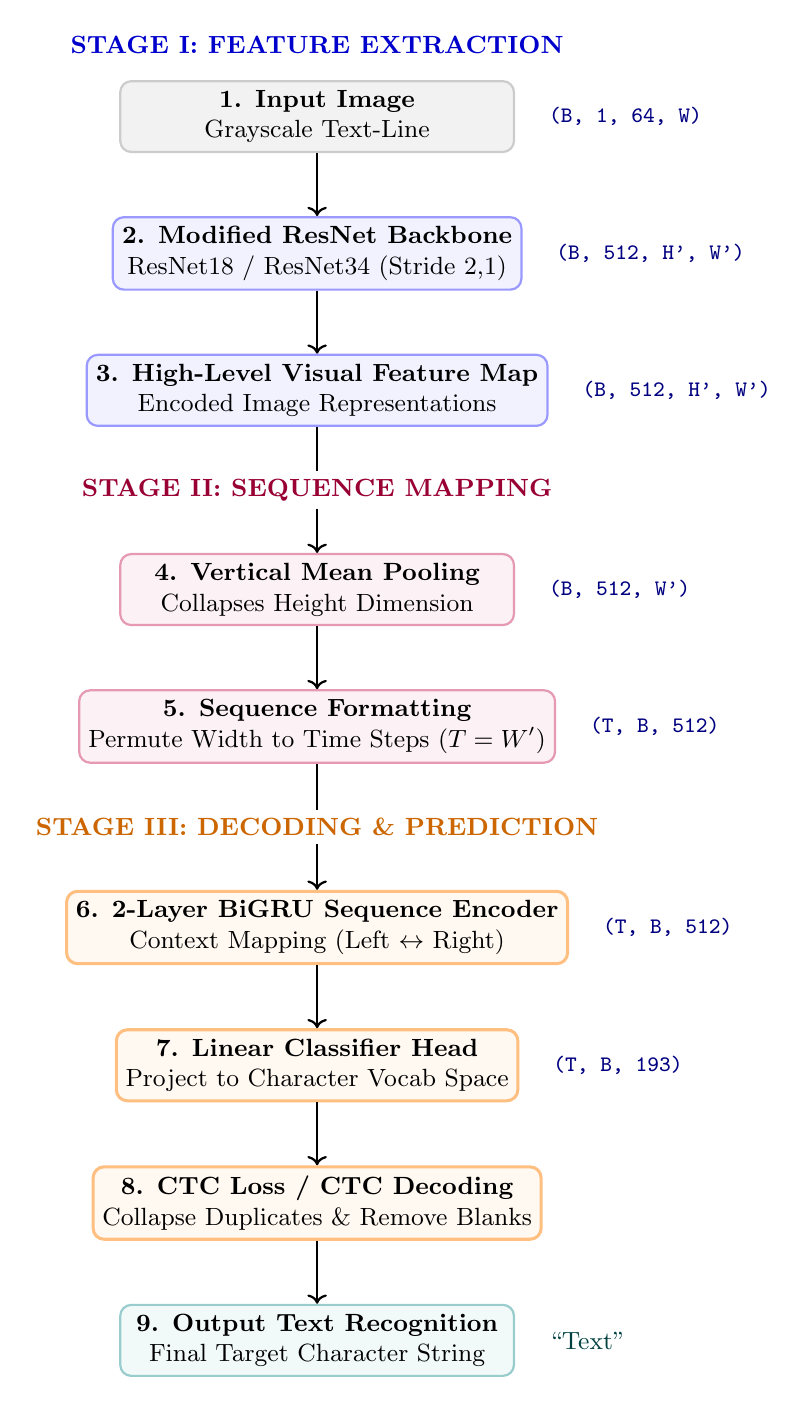
\begin{tikzpicture}[
    thick,
    node distance=0.8cm and 1.2cm,
    base/.style={
        draw, 
        minimum width=5.0cm, 
        minimum height=0.8cm, 
        align=center, 
        font=\small\bfseries, 
        rounded corners=4pt,
        line width=0.8pt
    },
    input/.style={base, fill=gray!10, draw=gray!40},
    vision/.style={base, fill=blue!5, draw=blue!40},
    seq_proc/.style={base, fill=purple!5, draw=purple!40},
    recog/.style={base, fill=orange!5, draw=orange!50, line width=1.1pt},
    output/.style={base, fill=teal!5, draw=teal!40},
    shape_node/.style={font=\footnotesize\ttfamily\color{blue!50!black}, anchor=west},
    stage_label/.style={font=\small\bfseries, fill=white, inner sep=3pt} 
]

    % STAGE I HEADER
    \node[font=\small\bfseries\color{blue!80!black}] (h1) {STAGE I: FEATURE EXTRACTION};
    
    \node[input, below=0.2cm of h1] (in) {1. Input Image\\{\normalfont Grayscale Text-Line}};
    \node[shape_node] (s_in) at (in.east) [xshift=0.3cm] {(B, 1, 64, W)};
    
    \node[vision, below=of in] (cnn) {2. Modified ResNet Backbone\\{\normalfont ResNet18 / ResNet34 (Stride 2,1)}};
    \node[shape_node] (s_cnn) at (cnn.east) [xshift=0.3cm] {(B, 512, H', W')};
    
    \node[vision, below=of cnn] (fmap) {3. High-Level Visual Feature Map\\{\normalfont Encoded Image Representations}};
    \node[shape_node] (s_fmap) at (fmap.east) [xshift=0.3cm] {(B, 512, H', W')};
    
    \node[seq_proc, below=1.6cm of fmap] (vpool) {4. Vertical Mean Pooling\\{\normalfont Collapses Height Dimension}};
    \node[shape_node] (s_vpool) at (vpool.east) [xshift=0.3cm] {(B, 512, W')};
    
    \node[seq_proc, below=of vpool] (format) {5. Sequence Formatting\\{\normalfont Permute Width to Time Steps ($T = W'$)}};
    \node[shape_node] (s_format) at (format.east) [xshift=0.3cm] {(T, B, 512)};
    
    \node[recog, below=1.6cm of format] (bigru) {6. 2-Layer BiGRU Sequence Encoder\\{\normalfont Context Mapping (Left $\leftrightarrow$ Right)}};
    \node[shape_node] (s_bigru) at (bigru.east) [xshift=0.3cm] {(T, B, 512)};
    
    \node[recog, below=of bigru] (linear) {7. Linear Classifier Head\\{\normalfont Project to Character Vocab Space}};
    \node[shape_node] (s_linear) at (linear.east) [xshift=0.3cm] {(T, B, 193)};
    
    \node[recog, below=of linear] (ctc) {8. CTC Loss / CTC Decoding\\{\normalfont Collapse Duplicates \& Remove Blanks}};
    
    \node[output, below=of ctc] (out) {9. Output Text Recognition\\{\normalfont Final Target Character String}};
    \node[shape_node, font=\small\color{teal!50!black}] (s_out) at (out.east) [xshift=0.3cm] {``Text''};

    \draw[->] (in) -- (cnn);
    \draw[->] (cnn) -- (fmap);
    \draw[->] (fmap) -- (vpool);   
    \draw[->] (vpool) -- (format);
    \draw[->] (format) -- (bigru); 
    \draw[->] (bigru) -- (linear);
    \draw[->] (linear) -- (ctc);
    \draw[->] (ctc) -- (out);

    \path (fmap) -- node[stage_label, text=purple!80!black] {STAGE II: SEQUENCE MAPPING} (vpool);
    \path (format) -- node[stage_label, text=orange!80!black] {STAGE III: DECODING \& PREDICTION} (bigru);

\end{tikzpicture}%
}
\caption{High-level CRNN architecture flow diagram. Each box is a processing stage; all stages are identical between the ResNet34 and ResNet18 variants.}
\label{fig:architecture}
\end{figure}

We adopt ResNet~\cite{he2016} variants adapted for grayscale input. Both
ResNet34 (16 residual blocks, 3+4+6+3) and ResNet18 (8 residual blocks, 2+2+2+2)
use the same asymmetric stride and vertical pooling strategies. On Khmer scene
text (KhmerST), ResNet-based models improve accuracy by $\sim$16.7\% relative
to VGG counterparts~\cite{vitou2026}.

\begin{figure*}[t]
\centering
\resizebox{0.95\linewidth}{!}{%
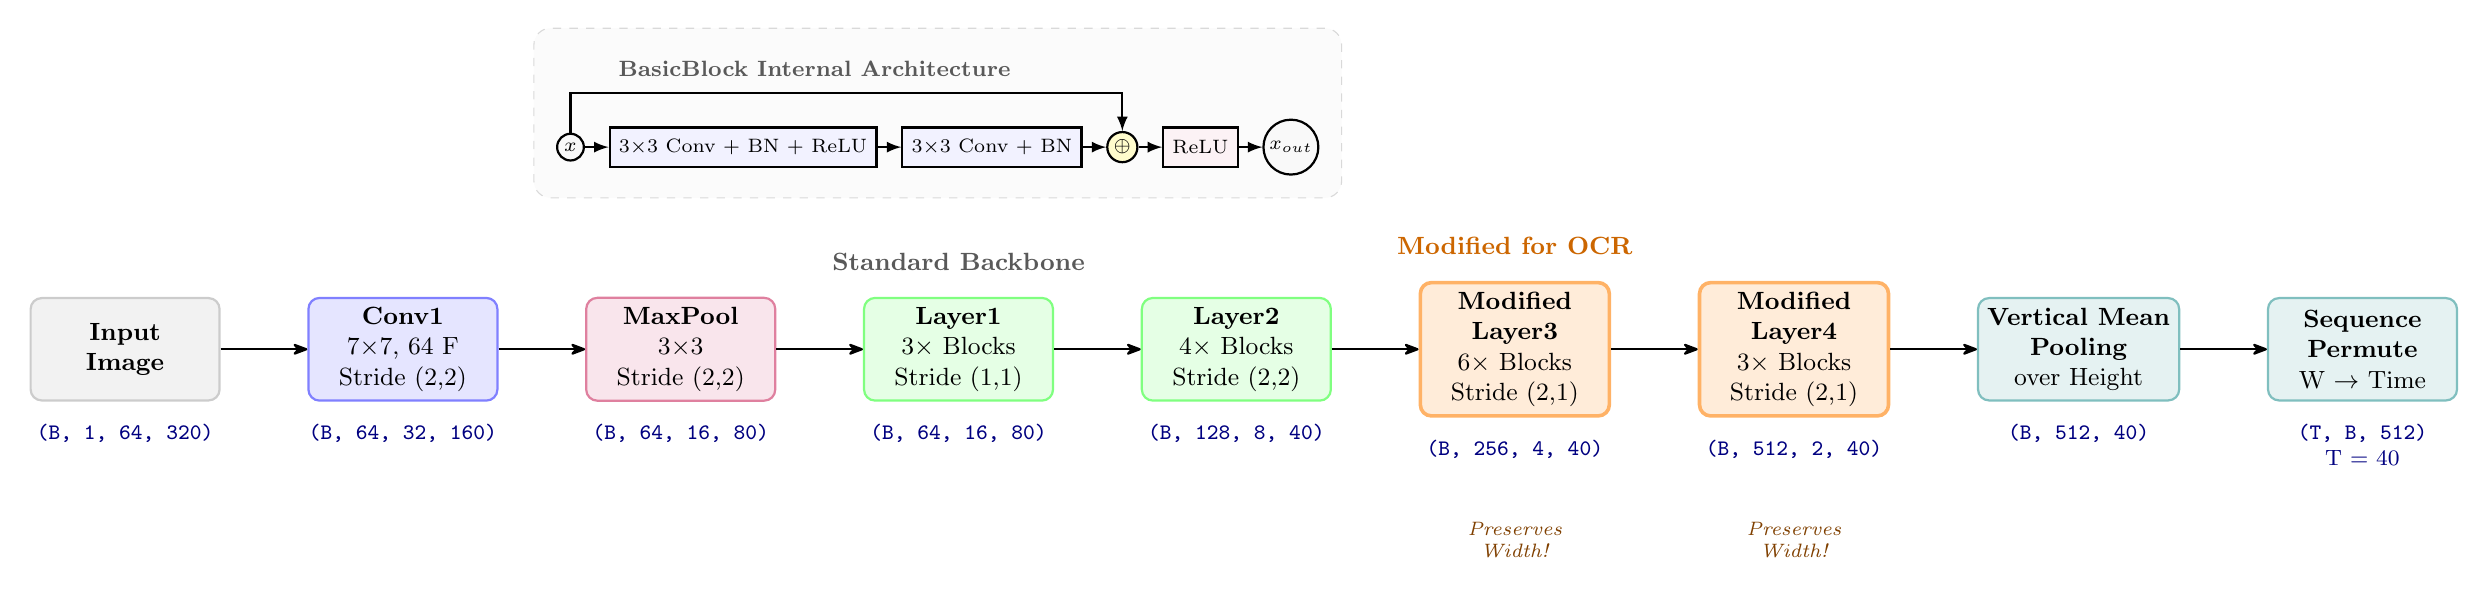
\begin{tikzpicture}[
    thick,
    node distance=1.0cm and 1.1cm,
    base/.style={draw, minimum width=2.4cm, minimum height=1.3cm, align=center, font=\small\bfseries, rounded corners=4pt, line width=0.8pt},
    input/.style={base, fill=gray!10, draw=gray!40},
    conv/.style={base, fill=blue!10, draw=blue!50},
    pool/.style={base, fill=purple!10, draw=purple!50},
    normal_res/.style={base, fill=green!10, draw=green!50},
    mod_res/.style={base, fill=orange!15, draw=orange!60, line width=1.3pt},
    post/.style={base, fill=teal!10, draw=teal!50},
    shape_node/.style={font=\footnotesize\ttfamily\color{blue!50!black}, align=center},
    note_node/.style={font=\scriptsize\itshape\color{orange!50!black}, align=center},
    >={Stealth[round]}
]
    \node[input] (in) {Input\\Image};
    \node[shape_node, below=0.15cm of in] (s_in) {(B, 1, 64, 320)};
    
    \node[conv, right=of in] (conv1) {Conv1\\{\normalfont 7$\times$7, 64 F}\\\normalfont Stride (2,2)};
    \node[shape_node, below=0.15cm of conv1] (s_c1) {(B, 64, 32, 160)};
    
    \node[pool, right=of conv1] (maxpool) {MaxPool\\{\normalfont 3$\times$3}\\\normalfont Stride (2,2)};
    \node[shape_node, below=0.15cm of maxpool] (s_mp) {(B, 64, 16, 80)};
    
    \node[normal_res, right=of maxpool] (lay1) {Layer1\\{\normalfont 3$\times$ Blocks}\\\normalfont Stride (1,1)};
    \node[shape_node, below=0.15cm of lay1] (s_l1) {(B, 64, 16, 80)};
    
    \node[normal_res, right=of lay1] (lay2) {Layer2\\{\normalfont 4$\times$ Blocks}\\\normalfont Stride (2,2)};
    \node[shape_node, below=0.15cm of lay2] (s_l2) {(B, 128, 8, 40)};
    
    \node[mod_res, right=of lay2] (lay3) {Modified\\Layer3\\{\normalfont 6$\times$ Blocks}\\\normalfont Stride (2,1)};
    \node[shape_node, below=0.15cm of lay3] (s_l3) {(B, 256, 4, 40)};
    \node[note_node, below=0.55cm of s_l3] (n_l3) {Preserves\\Width!};
    
    \node[mod_res, right=of lay3] (lay4) {Modified\\Layer4\\{\normalfont 3$\times$ Blocks}\\\normalfont Stride (2,1)};
    \node[shape_node, below=0.15cm of lay4] (s_l4) {(B, 512, 2, 40)};
    \node[note_node, below=0.55cm of s_l4] (n_l4) {Preserves\\Width!};
    
    \node[post, right=of lay4] (pool2d) {Vertical Mean\\Pooling\\{\normalfont over Height}};
    \node[shape_node, below=0.15cm of pool2d] (s_p2d) {(B, 512, 40)};
    
    \node[post, right=of pool2d] (reshape) {Sequence\\Permute\\{\normalfont W $\to$ Time}};
    \node[shape_node, below=0.15cm of reshape] (s_resh) {(T, B, 512)\\{\normalfont T = 40}};

    \draw[->] (in) -- (conv1);
    \draw[->] (conv1) -- (maxpool);
    \draw[->] (maxpool) -- (lay1);
    \draw[->] (lay1) -- (lay2);
    \draw[->] (lay2) -- (lay3);
    \draw[->] (lay3) -- (lay4);
    \draw[->] (lay4) -- (pool2d);
    \draw[->] (pool2d) -- (reshape);

    \node[font=\small\bfseries\color{gray!70!black}, above=0.2cm of lay1] {Standard Backbone};
    \node[font=\small\bfseries\color{orange!80!black}, above=0.2cm of lay3] {Modified for OCR};

    \begin{scope}[shift={($(maxpool.north) + (-1.4, 1.7)$)}]
        \node[font=\footnotesize\bfseries, text=gray!70!black] (bbtitle) at (3.1, 1.2) {BasicBlock Internal Architecture};
        \node[circle, draw, fill=gray!5, inner sep=1.5pt, font=\scriptsize] (xi) at (0, 0.2) {$x$};
        \node[draw, fill=blue!5, font=\scriptsize, minimum height=0.5cm, right=0.3cm of xi] (c1) {3$\times$3 Conv + BN + ReLU};
        \node[draw, fill=blue!5, font=\scriptsize, minimum height=0.5cm, right=0.3cm of c1] (c2) {3$\times$3 Conv + BN};
        \node[circle, draw, fill=yellow!20, font=\scriptsize, inner sep=1pt, right=0.3cm of c2] (add) {$\oplus$};
        \node[draw, fill=purple!5, font=\scriptsize, minimum height=0.5cm, right=0.3cm of add] (r2) {ReLU};
        \node[circle, draw, fill=gray!5, inner sep=1.5pt, font=\scriptsize, right=0.3cm of r2] (xo) {$x_{out}$};
        \draw[->, >=latex] (xi) -- (c1);
        \draw[->, >=latex] (c1) -- (c2);
        \draw[->, >=latex] (c2) -- (add);
        \draw[->, >=latex] (add) -- (r2);
        \draw[->, >=latex] (r2) -- (xo);
        \draw[->, >=latex] (xi.north) -- ++(0,0.5) node(skiptop){} -| (add.north);
        \begin{pgfonlayer}{background}
            \node[draw=gray!30, fill=gray!3, dashed, rounded corners=6pt, inner sep=8pt, fit=(bbtitle) (xi) (xo) (skiptop) (c1) (c2) (add) (r2)] {};
        \end{pgfonlayer}
    \end{scope}
\end{tikzpicture}%
}
\caption{Detailed ResNet34 backbone internal architecture layout. Specially modified stride parameters in Layers 3 and 4 maintain sequence width resolution.}
\label{fig:resnet34}
\end{figure*}

\begin{figure*}[t]
\centering
\resizebox{0.95\linewidth}{!}{%
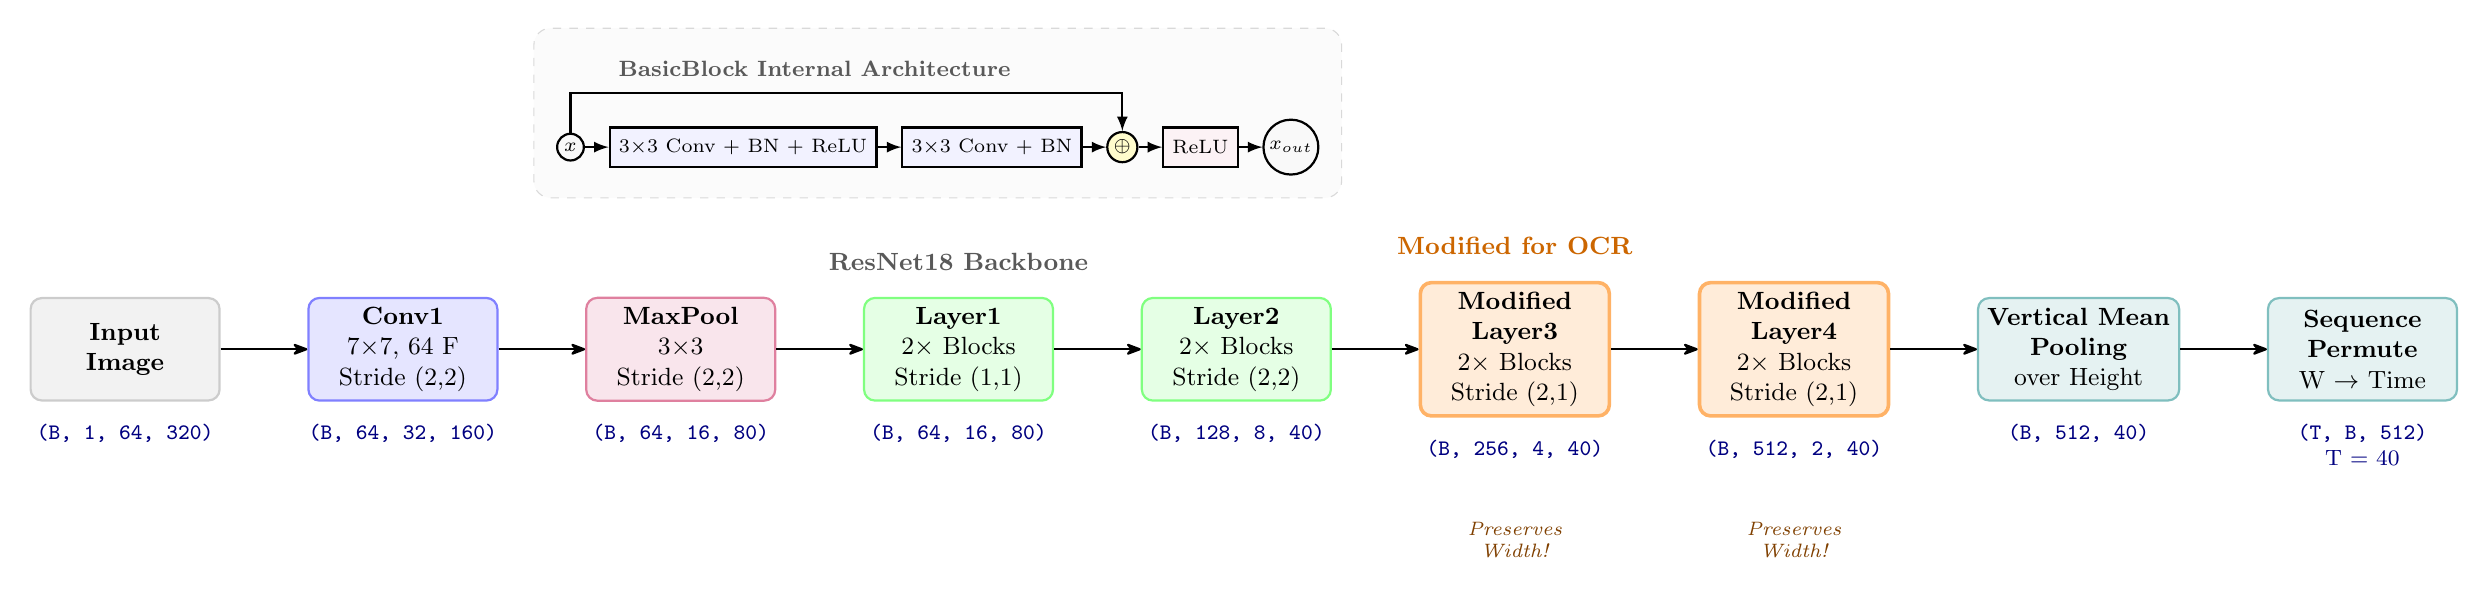
\begin{tikzpicture}[
    thick,
    node distance=1.0cm and 1.1cm,
    base/.style={draw, minimum width=2.4cm, minimum height=1.3cm, align=center, font=\small\bfseries, rounded corners=4pt, line width=0.8pt},
    input/.style={base, fill=gray!10, draw=gray!40},
    conv/.style={base, fill=blue!10, draw=blue!50},
    pool/.style={base, fill=purple!10, draw=purple!50},
    normal_res/.style={base, fill=green!10, draw=green!50},
    mod_res/.style={base, fill=orange!15, draw=orange!60, line width=1.3pt},
    post/.style={base, fill=teal!10, draw=teal!50},
    shape_node/.style={font=\footnotesize\ttfamily\color{blue!50!black}, align=center},
    note_node/.style={font=\scriptsize\itshape\color{orange!50!black}, align=center},
    >={Stealth[round]}
]
    \node[input] (in) {Input\\Image};
    \node[shape_node, below=0.15cm of in] (s_in) {(B, 1, 64, 320)};
    
    \node[conv, right=of in] (conv1) {Conv1\\{\normalfont 7$\times$7, 64 F}\\\normalfont Stride (2,2)};
    \node[shape_node, below=0.15cm of conv1] (s_c1) {(B, 64, 32, 160)};
    
    \node[pool, right=of conv1] (maxpool) {MaxPool\\{\normalfont 3$\times$3}\\\normalfont Stride (2,2)};
    \node[shape_node, below=0.15cm of maxpool] (s_mp) {(B, 64, 16, 80)};
    
    \node[normal_res, right=of maxpool] (lay1) {Layer1\\{\normalfont 2$\times$ Blocks}\\\normalfont Stride (1,1)};
    \node[shape_node, below=0.15cm of lay1] (s_l1) {(B, 64, 16, 80)};
    
    \node[normal_res, right=of lay1] (lay2) {Layer2\\{\normalfont 2$\times$ Blocks}\\\normalfont Stride (2,2)};
    \node[shape_node, below=0.15cm of lay2] (s_l2) {(B, 128, 8, 40)};
    
    \node[mod_res, right=of lay2] (lay3) {Modified\\Layer3\\{\normalfont 2$\times$ Blocks}\\\normalfont Stride (2,1)};
    \node[shape_node, below=0.15cm of lay3] (s_l3) {(B, 256, 4, 40)};
    \node[note_node, below=0.55cm of s_l3] (n_l3) {Preserves\\Width!};
    
    \node[mod_res, right=of lay3] (lay4) {Modified\\Layer4\\{\normalfont 2$\times$ Blocks}\\\normalfont Stride (2,1)};
    \node[shape_node, below=0.15cm of lay4] (s_l4) {(B, 512, 2, 40)};
    \node[note_node, below=0.55cm of s_l4] (n_l4) {Preserves\\Width!};
    
    \node[post, right=of lay4] (pool2d) {Vertical Mean\\Pooling\\{\normalfont over Height}};
    \node[shape_node, below=0.15cm of pool2d] (s_p2d) {(B, 512, 40)};
    
    \node[post, right=of pool2d] (reshape) {Sequence\\Permute\\{\normalfont W $\to$ Time}};
    \node[shape_node, below=0.15cm of reshape] (s_resh) {(T, B, 512)\\{\normalfont T = 40}};

    \draw[->] (in) -- (conv1);
    \draw[->] (conv1) -- (maxpool);
    \draw[->] (maxpool) -- (lay1);
    \draw[->] (lay1) -- (lay2);
    \draw[->] (lay2) -- (lay3);
    \draw[->] (lay3) -- (lay4);
    \draw[->] (lay4) -- (pool2d);
    \draw[->] (pool2d) -- (reshape);

    \node[font=\small\bfseries\color{gray!70!black}, above=0.2cm of lay1] {ResNet18 Backbone};
    \node[font=\small\bfseries\color{orange!80!black}, above=0.2cm of lay3] {Modified for OCR};

    \begin{scope}[shift={($(maxpool.north) + (-1.4, 1.7)$)}]
        \node[font=\footnotesize\bfseries, text=gray!70!black] (bbtitle) at (3.1, 1.2) {BasicBlock Internal Architecture};
        \node[circle, draw, fill=gray!5, inner sep=1.5pt, font=\scriptsize] (xi) at (0, 0.2) {$x$};
        \node[draw, fill=blue!5, font=\scriptsize, minimum height=0.5cm, right=0.3cm of xi] (c1) {3$\times$3 Conv + BN + ReLU};
        \node[draw, fill=blue!5, font=\scriptsize, minimum height=0.5cm, right=0.3cm of c1] (c2) {3$\times$3 Conv + BN};
        \node[circle, draw, fill=yellow!20, font=\scriptsize, inner sep=1pt, right=0.3cm of c2] (add) {$\oplus$};
        \node[draw, fill=purple!5, font=\scriptsize, minimum height=0.5cm, right=0.3cm of add] (r2) {ReLU};
        \node[circle, draw, fill=gray!5, inner sep=1.5pt, font=\scriptsize, right=0.3cm of r2] (xo) {$x_{out}$};
        \draw[->, >=latex] (xi) -- (c1);
        \draw[->, >=latex] (c1) -- (c2);
        \draw[->, >=latex] (c2) -- (add);
        \draw[->, >=latex] (add) -- (r2);
        \draw[->, >=latex] (r2) -- (xo);
        \draw[->, >=latex] (xi.north) -- ++(0,0.5) node(skiptop){} -| (add.north);
        \begin{pgfonlayer}{background}
            \node[draw=gray!30, fill=gray!3, dashed, rounded corners=6pt, inner sep=8pt, fit=(bbtitle) (xi) (xo) (skiptop) (c1) (c2) (add) (r2)] {};
        \end{pgfonlayer}
    \end{scope}
\end{tikzpicture}%
}
\caption{Detailed ResNet18 backbone internal architecture layout. Block counts are reduced to 2 per layer, allowing faster throughput compared to ResNet34.}
\label{fig:resnet18}
\end{figure*}

\subsubsection{Asymmetric Stride Pooling}

Following Shi \emph{et al.}~\cite{shi2017}, we apply asymmetric pooling: layers
1--2 use standard $2\times2$ stride, while layers 3--4 use $2\times1$ stride
(stride 2 vertically, 1 horizontally). This preserves horizontal resolution and
ensures the CTC time steps $T \geq$ label length $L$:
\begin{itemize}
  \item Layer 1: $W/2$;\quad Layer 2: $W/4$;\quad Layers 3--4: $W/4$ (no
        horizontal reduction).
\end{itemize}
Buoy \emph{et al.}~\cite{buoy2023} similarly caution that naive width
downsampling makes subscripts and diacritics ``blur out.''

\subsubsection{Vertical Mean Pooling}

After the final ResNet layer, we apply vertical mean pooling
($\texttt{f.mean(dim=2)}$) to collapse the height dimension, producing a 1D
feature sequence of shape $(T, 512)$.

\subsection{Recurrent Module: Bidirectional GRU}

The feature sequence is fed into a 2-layer bidirectional GRU~\cite{cho2014}
with hidden size 256 and dropout 0.2. BiGRU is chosen over BiLSTM for its
$\sim$25\% fewer parameters, faster training, and competitive accuracy.

\begin{figure}[htbp]
\centering
\resizebox{0.95\columnwidth}{!}{%
\begin{tikzpicture}[
    thick,
    node distance=1.0cm and 1.8cm,
    cell/.style={draw, minimum width=2.2cm, minimum height=9mm, align=center, font=\small\bfseries, rounded corners=2pt},
    fwd/.style={cell, fill=blue!10, draw=blue!60, text=blue!50!black},
    bwd/.style={cell, fill=orange!5, draw=orange!60, text=orange!50!black},
    io/.style={draw, circle, minimum size=7mm, inner sep=0pt, draw=blue!50, fill=white, font=\small},
    label/.style={font=\small\itshape\bfseries},
    >={Stealth[round]}
]
    % Time Step t-1
    \node[io] (x1) at (0,0) {$x_{t-1}$};
    \node[fwd] (f1) [above=1.2cm of x1] {Forward\\GRU};
    \node[bwd] (b1) at ($(f1) + (1.3, 1.5)$) {Backward\\GRU};
    \node[io] (c1) at ($(f1.north) + (0, 2.5)$) {$\oplus$};
    \node[above=0.2cm of c1, font=\small] (y1) {$y_{t-1}$};

    % Time Step t
    \node[io] (x2) at (4.0,0) {$x_{t}$};
    \node[fwd] (f2) [above=1.2cm of x2] {Forward\\GRU};
    \node[bwd] (b2) at ($(f2) + (1.3, 1.5)$) {Backward\\GRU};
    \node[io] (c2) at ($(f2.north) + (0, 2.5)$) {$\oplus$};
    \node[above=0.2cm of c2, font=\small] (y2) {$y_{t}$};

    % Time Step t+1
    \node[io] (x3) at (8.0,0) {$x_{t+1}$};
    \node[fwd] (f3) [above=1.2cm of x3] {Forward\\GRU};
    \node[bwd] (b3) at ($(f3) + (1.3, 1.5)$) {Backward\\GRU};
    \node[io] (c3) at ($(f3.north) + (0, 2.5)$) {$\oplus$};
    \node[above=0.2cm of c3, font=\small] (y3) {$y_{t+1}$};

    \node[label, below=0.4cm of x2] {Input Layer};
    \node[label, above=0.6cm of c2] {Output Layer};

    \begin{scope}[draw=orange!80, -{Stealth[round]}, thick]
        \foreach \i in {1,2,3} {
            \draw (x\i) -- (f\i);
            \draw (f\i) -- (c\i);
            \draw (c\i) -- (y\i);
            \draw ($(x\i.north)!0.4!(f\i.south)$) -| (b\i.south);
            \draw (b\i.north) |- (c\i.east);
        }
        \draw [dashed] ($(f1.west) - (0.6,0)$) -- (f1.west);
        \draw (f1) -- (f2);
        \draw (f2) -- (f3);
        \draw [dashed] (f3.east) -- ($(f3.east) + (0.6,0)$);
        \draw [dashed] ($(b3.east) + (0.6,0)$) -- (b3.east);
        \draw (b3) -- (b2);
        \draw (b2) -- (b1);
        \draw [dashed] (b1.west) -- ($(b1.west) - (0.6,0)$);
    \end{scope}

    \begin{backgroundlayer}
        \node[draw=blue!40, dashed, rounded corners=12pt, inner sep=15pt, fit=(f1) (b3), line width=1pt] (bbox) {};
        \node[label, align=center, rotate=90, left=0.4cm of bbox.west] {Bidirectional\\Layer};
    \end{backgroundlayer}
\end{tikzpicture}%
}
\caption{Detailed internal structure of the 2-layer BiGRU module. Each layer is bidirectional: forward and backward GRU cells process the sequence in both directions and their outputs are concatenated at the summation nodes before output projection.}
\label{fig:bigru}
\end{figure}

\subsection{Classifier and CTC Decoding}

The GRU output is projected through a linear layer to size $|V| + 1$ (CTC blank
at index~0). We minimize the CTC loss~\cite{graves2006}:
\begin{equation}
\mathcal{L}_{\text{CTC}} = -\ln \sum_{\pi \in \mathcal{B}^{-1}(y)}
\prod_{t=1}^{T} p(\pi_t \mid x)
\end{equation}
During inference, best-path (greedy) decoding is used: argmax per time step
followed by blank removal and consecutive-character merging.

\section{EXPERIMENTS AND RESULTS}

\subsection{Experimental Setup}

\begin{table}[htbp]
\centering
\caption{Training hyperparameters.}
\label{tab:hyperparams}
\begin{tabularx}{\columnwidth}{@{}l X@{}} 
\toprule
\textbf{Component} & \textbf{Configuration} \\ 
\midrule
Backbone & ResNet34 / ResNet18 (1-channel, no pretrain) \\ 
Strides & Layers 1--2: (2,2); Layers 3--4: (2,1) \\ 
Vert.\ pool & Mean-pooling ($\texttt{f.mean(dim=2)}$) \\ 
RNN & 2-layer BiGRU, hidden 256, dropout 0.2 \\ 
Loss & CTC (blank=0, $\texttt{zero\_infinity=True}$)~\cite{graves2006} \\ 
Optimizer & AdamW, weight decay $1\times10^{-4}$ \\ 
LR & $1\times10^{-4}$ for the ResNet18 comparison run \\ 
Batch size & 256 (dynamic-width, grouped batching) \\ 
Augmentation & Rot. $\pm3^\circ$, Color jitter (B=0.2,C=0.2), Gauss. blur ($3\times3$, $\sigma\in[0.1,1.0]$), Rand.\ erasing ($p=0.4$, scale $[0.02,0.08]$) \\ 
\bottomrule
\end{tabularx}
\end{table}

Both ResNet34 and ResNet18 CRNN models were trained on the same 80/10/10 split.
The architectural difference is the CNN backbone depth; both use the same
vertical pooling, BiGRU sequence encoder, and CTC objective.
\subsection{Evaluation Protocols}

\paragraph{Primary metric:} Normalized Character Error Rate (CER)
\begin{equation}
\text{CER} = \frac{\text{edit\_distance}(\hat{y}, y)}{\max(|\hat{y}|, |y|)}
\end{equation}
where $\hat{y}$ is the predicted text and $y$ is the ground truth.

\paragraph{Secondary metric:} Exact Match Accuracy (EMA)
\begin{equation}
\text{EMA} = \frac{\text{\# perfectly matched samples}}{\text{total samples}}
\end{equation}

\subsection{Results}

\subsubsection{Overall Performance}

The final models (epoch~25) achieved the following on the held-out validation
set of 20,000 samples:

\begin{table}[htbp]
\centering
\caption{Final validation performance.}
\label{tab:results}
\begin{tabular}{@{}lcc@{}}
\toprule
\textbf{Metric} & \textbf{ResNet34 CRNN} & \textbf{ResNet18 CRNN} \\
\midrule
Validation CER           & 0.1635\% & 0.4325\% \\
Character Accuracy       & 99.8365\% & 99.5675\% \\
Exact Match Accuracy     & 95.695\% & 90.245\% \\
Final Validation Loss    & 0.0085 & 0.0189 \\
Final Test CER           & $\sim$0.18\% & 0.4509\% \\
Trainable Parameters     & 23,742,849 & 13,634,689 \\
\bottomrule
\end{tabular}
\end{table}

\begin{figure}[htbp]
\centering
\resizebox{\columnwidth}{!}{%
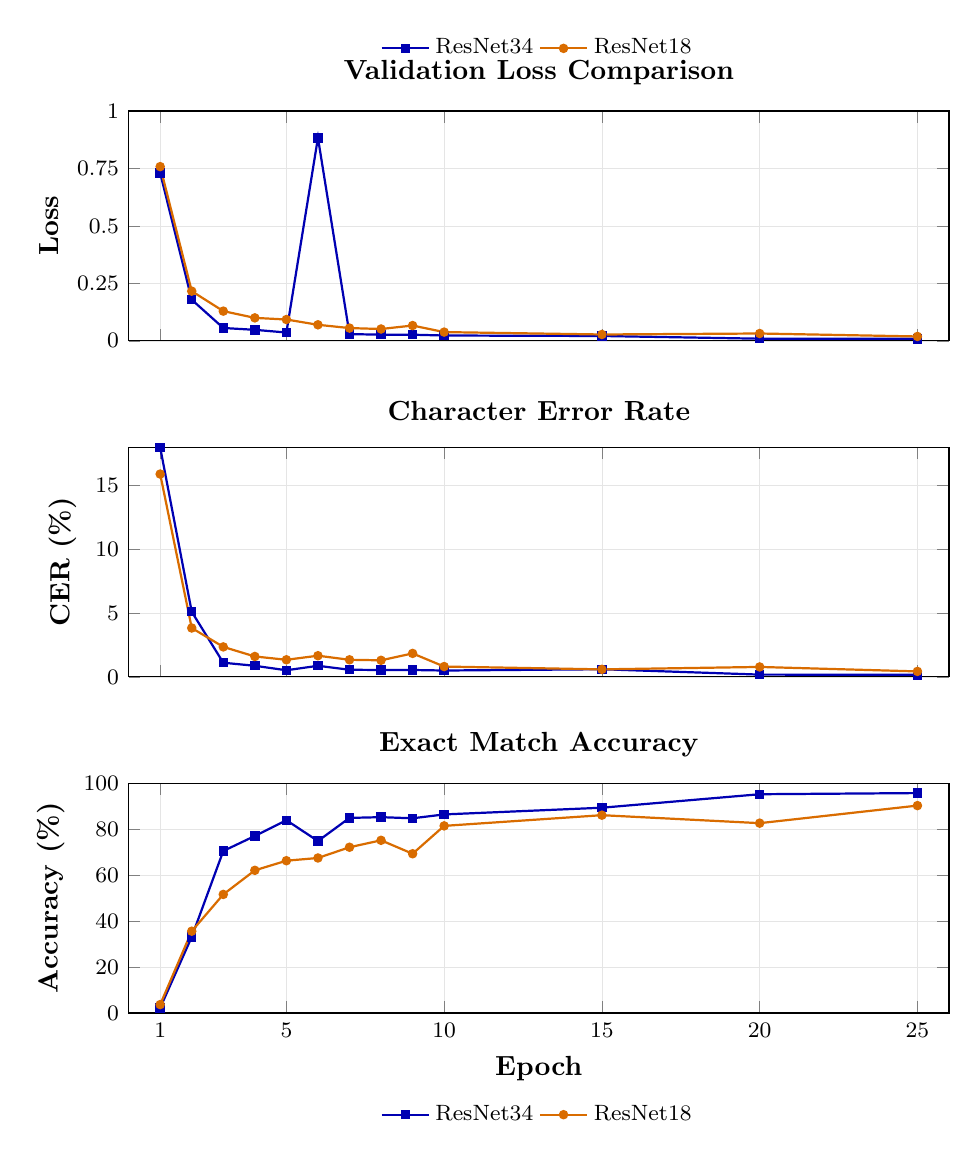
\begin{tikzpicture}
    \begin{groupplot}[
        group style={
            group size=1 by 3,
            vertical sep=1.35cm,
            xlabels at=edge bottom,
            xticklabels at=edge bottom
        },
        width=12cm,
        height=4.5cm,
        grid=both,
        grid style={line width=.1pt, draw=gray!10},
        major grid style={line width=.2pt, draw=gray!20},
        xmin=0, xmax=26,
        xtick={1,5,10,15,20,25},
        tick label style={font=\footnotesize},
        legend style={at={(0.5,1.18)}, anchor=south, legend columns=-1, font=\footnotesize, draw=none, fill=none}
    ]

    % --------------------------------------------------
    % CHART 1: VALIDATION LOSS
    % --------------------------------------------------
    \nextgroupplot[
        title={\bfseries Validation Loss Comparison},
        ylabel={\bfseries Loss},
        ymin=0, ymax=1.0,
        ytick={0,0.25,0.5,0.75,1.0}
    ]
    \addplot[color=blue!70!black, mark=square*, thick, mark size=1.3pt] coordinates {
        (1,0.729830) (2,0.178840) (3,0.055744) (4,0.047783) (5,0.036029)
        (6,0.883362) (7,0.029081) (8,0.026788) (9,0.026495) (10,0.023068)
        (15,0.020919) (20,0.009163) (25,0.008510)
    };
    \addlegendentry{ResNet34}

    \addplot[color=orange!85!black, mark=*, thick, mark size=1.3pt] coordinates {
        (1,0.757937) (2,0.216043) (3,0.129134) (4,0.099774) (5,0.092634)
        (6,0.069687) (7,0.055372) (8,0.051380) (9,0.066463) (10,0.037886)
        (15,0.027483) (20,0.031765) (25,0.018886)
    };
    \addlegendentry{ResNet18}

    % --------------------------------------------------
    % CHART 2: CER
    % --------------------------------------------------
    \nextgroupplot[
        title={\bfseries Character Error Rate},
        ylabel={\bfseries CER (\%)},
        ymin=0, ymax=18,
        ytick={0,5,10,15}
    ]
    \addplot[color=blue!70!black, mark=square*, thick, mark size=1.3pt] coordinates {
        (1,17.97) (2,5.10) (3,1.11) (4,0.87) (5,0.52) (6,0.87)
        (7,0.56) (8,0.54) (9,0.54) (10,0.50) (15,0.60) (20,0.18) (25,0.16)
    };

    \addplot[color=orange!85!black, mark=*, thick, mark size=1.3pt] coordinates {
        (1,15.89) (2,3.83) (3,2.35) (4,1.60) (5,1.34) (6,1.66)
        (7,1.34) (8,1.30) (9,1.84) (10,0.81) (15,0.59) (20,0.78) (25,0.43)
    };

    % --------------------------------------------------
    % CHART 3: EXACT MATCH ACCURACY
    % --------------------------------------------------
    \nextgroupplot[
        title={\bfseries Exact Match Accuracy},
        xlabel={\bfseries Epoch},
        ylabel={\bfseries Accuracy (\%)},
        ymin=0, ymax=100,
        ytick={0,20,40,60,80,100},
        legend style={at={(0.5,-0.35)}, anchor=north, legend columns=-1, font=\footnotesize, draw=none}
    ]
    \addplot[color=blue!70!black, mark=square*, thick, mark size=1.3pt] coordinates {
        (1,2.23) (2,33.11) (3,70.50) (4,77.03) (5,83.89) (6,74.83)
        (7,84.90) (8,85.22) (9,84.73) (10,86.41) (15,89.33) (20,95.20) (25,95.70)
    };
    \addlegendentry{ResNet34}

    \addplot[color=orange!85!black, mark=*, thick, mark size=1.3pt] coordinates {
        (1,3.66) (2,35.59) (3,51.60) (4,62.08) (5,66.27) (6,67.46)
        (7,72.13) (8,75.15) (9,69.30) (10,81.43) (15,86.08) (20,82.61) (25,90.25)
    };
    \addlegendentry{ResNet18}

    \end{groupplot}
\end{tikzpicture}%
}
\caption{Validation metric comparison for ResNet34 and ResNet18 CRNN models: validation loss, character error rate (CER), and exact match accuracy, generated directly in LaTeX using pgfplots.}
\label{fig:resnet-comparison}
\end{figure}

Despite having 1.74$\times$ fewer parameters, the ResNet18 CRNN model remains highly
competitive, reaching 0.4509\% test CER. The deeper ResNet34 remains more
accurate, reaching approximately 0.18\% test CER and 95.695\% validation exact
match accuracy; ResNet18 reaches 90.245\% validation exact match accuracy. This suggests that backbone depth still improves fine-grained
Khmer recognition, but a smaller ResNet18 backbone is a practical lightweight
alternative.

\subsubsection{Training Dynamics}

Figure~\ref{fig:curves} shows the training curves. Key observations:
\begin{itemize}
  \item \textbf{Rapid convergence (epochs 1--3):} Validation loss dropped from
        0.73 to 0.06, CER from 17.97\% to 1.11\%, accuracy from 2.23\% to
        70.50\%.
  \item \textbf{Loss spike at epoch 6:} Validation loss briefly spiked to 0.88
        (CER 0.87\%), likely due to a difficult batch; the model recovered
        within one epoch.
  \item \textbf{Late-stage refinement:} ResNet34 improved from 0.60\% CER at
        epoch~15 to 0.16\% CER at epoch~25, while ResNet18 improved from
        0.59\% to 0.43\% CER over the same checkpoint interval.
\end{itemize}

\begin{figure}[htbp]
\centering
\resizebox{\columnwidth}{!}{%
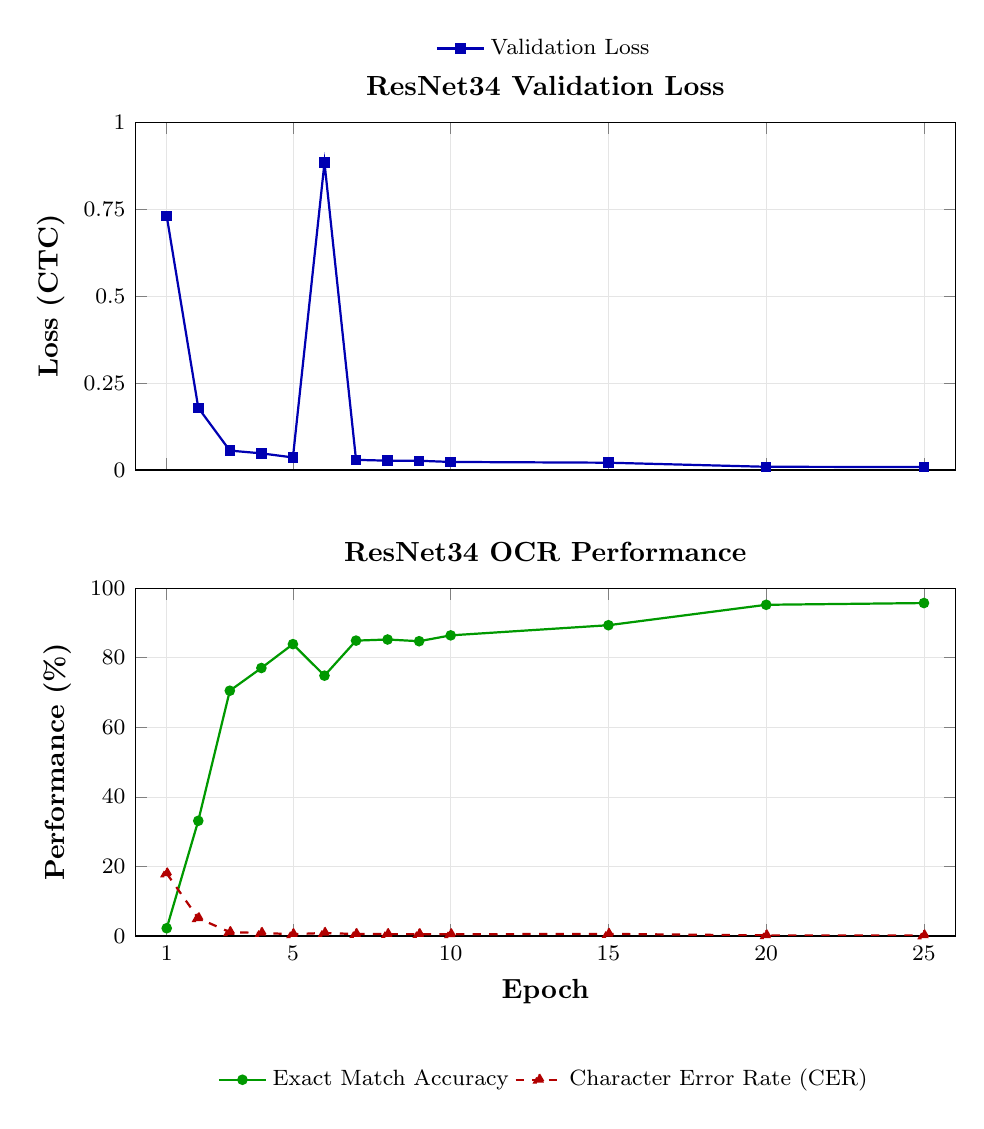
\begin{tikzpicture}
    \begin{groupplot}[
        group style={
            group size=1 by 2,
            vertical sep=1.5cm,
            xlabels at=edge bottom,
            xticklabels at=edge bottom
        },
        width=12cm,
        height=6cm,
        grid=both,
        grid style={line width=.1pt, draw=gray!10},
        major grid style={line width=.2pt, draw=gray!20},
        xmin=0, xmax=26,
        xtick={1,5,10,15,20,25},
        tick label style={font=\footnotesize}
    ]

    % --------------------------------------------------
    % CHART 1: VALIDATION LOSS
    % --------------------------------------------------
    \nextgroupplot[
        title={\bfseries ResNet34 Validation Loss},
        ylabel={\bfseries Loss (CTC)},
        ylabel style={align=center},
        ymin=0, ymax=1.0,
        ytick={0, 0.25, 0.5, 0.75, 1.0},
        legend style={at={(0.5,1.15)}, anchor=south, legend columns=-1, font=\footnotesize, draw=none, fill=none}
    ]
    \addplot[color=blue!70!black, mark=square*, thick, mark size=1.5pt] coordinates {
        (1, 0.729830) (2, 0.178840) (3, 0.055744) (4, 0.047783)
        (5, 0.036029) (6, 0.883362) (7, 0.029081) (8, 0.026788)
        (9, 0.026495) (10, 0.023068) (15, 0.020919) (20, 0.009163) (25, 0.008510)
    };
    \addlegendentry{Validation Loss}

    % --------------------------------------------------
    % CHART 2: ACCURACY AND CER
    % --------------------------------------------------
    \nextgroupplot[
        title={\bfseries ResNet34 OCR Performance},
        xlabel={\bfseries Epoch},
        ylabel={\bfseries Performance (\%)},
        ymin=0, ymax=100,
        ytick={0, 20, 40, 60, 80, 100},
        legend style={at={(0.5,-0.35)}, anchor=north, legend columns=-1, font=\footnotesize, draw=none}
    ]

    \addplot[color=green!60!black, mark=*, thick, mark size=1.5pt] coordinates {
        (1, 2.23) (2, 33.11) (3, 70.50) (4, 77.03)
        (5, 83.89) (6, 74.83) (7, 84.90) (8, 85.22)
        (9, 84.73) (10, 86.41) (15, 89.33) (20, 95.20) (25, 95.70)
    };
    \addlegendentry{Exact Match Accuracy}

    \addplot[color=red!70!black, mark=triangle*, thick, dashed, mark size=2pt] coordinates {
        (1, 17.97) (2, 5.10) (3, 1.11) (4, 0.87)
        (5, 0.52) (6, 0.87) (7, 0.56) (8, 0.54)
        (9, 0.54) (10, 0.50) (15, 0.60) (20, 0.18) (25, 0.16)
    };
    \addlegendentry{Character Error Rate (CER)}

    \end{groupplot}
\end{tikzpicture}%
}
\caption{ResNet34 training progress curves across 25 epochs: validation loss, character error rate (CER), and exact match accuracy, generated directly in LaTeX using pgfplots.}
\label{fig:curves}
\end{figure}

\subsubsection{Error Analysis}

Despite the low CER, the remaining 4.30\% of lines with errors exhibit
consistent patterns:
\begin{itemize}
  \item \textbf{Confusable vowel diacritics:} Pairs such as {\khmerfont ឹ}/{\khmerfont ឺ} (short/long u)
        and {\khmerfont ែ}/{\khmerfont េ} (ae/e) are occasionally swapped in low-contrast renderings.
  \item \textbf{Subscript consonant omissions:} In densely stacked clusters
        with 3+ characters, the model occasionally drops a medial subscript.
  \item \textbf{Padding sensitivity:} Lines with extreme tight padding show
        marginally higher CER.
\end{itemize}
These errors are consistent with known Khmer OCR challenges~\cite{buoy2023}
and are expected to decrease with larger datasets and real-image fine-tuning.

%==============================================================================
% V. CONCLUSION
%==============================================================================
\section{CONCLUSION}

We presented a comparative study of two CRNN architectures for Khmer OCR, namely the
ResNet34 CRNN (23.7M params) and ResNet18 CRNN (13.6M params) models, trained with
identical sequence modelling and data pipelines. ResNet34 achieved the best
performance, with 0.1635\% validation CER and 95.695\% exact match accuracy.
ResNet18 achieved 0.4325\% validation CER and 90.245\% exact match accuracy with
1.74$\times$ fewer parameters, demonstrating a useful accuracy--efficiency
trade-off for resource-constrained deployment.

Future work includes: larger and more diverse datasets (real scanned documents,
handwriting); YOLO-based text detection for end-to-end pipelines; attention
decoder and language model post-correction; real-world evaluation to close the
synthetic-to-real domain gap; and class-weighted losses (Focal CTC) to address
rare diacritic errors.
%------------------------------------------------------------------------------
% ACKNOWLEDGMENT
%------------------------------------------------------------------------------
\section*{ACKNOWLEDGMENT}
The authors would like to thank Dr. Dona Valy for teaching the Advanced Machine Learning course, and for his guidance and support.

%------------------------------------------------------------------------------
% REFERENCES
%------------------------------------------------------------------------------
\begin{thebibliography}{00}

\bibitem{buoy2023}
R.~Buoy, M.~Iwamura, S.~Srun, and K.~Kise,
``Toward a low-resource non-latin-complete baseline: An exploration of Khmer
optical character recognition,'' \textit{IEEE Access}, vol.~11,
pp.~138\,544--138\,566, 2023.

\bibitem{buoy2025}
R.~Buoy, S.~Chenda, N.~Taing, and M.~Kong,
``Addressing the attention drift problem for Khmer long textline recognition,''
\textit{Int. J. Document Analysis and Recognition (IJDAR)}, 2025.

\bibitem{nom2024}
V.~Nom, S.~Bakkali, M.~M.~Luqman, M.~Coustaty, and J.-M.~Ogier,
``KhmerST: A low-resource Khmer scene text detection and recognition benchmark,''
in \textit{Proc. Asian Conf. Computer Vision (ACCV)}, 2024.

\bibitem{vitou2026}
S.~Vitou and E.~Koungmeng,
``KPTMA2026: A real-world bilingual Khmer-English OCR benchmark with lightweight
CRNN baselines,'' 2026.

\bibitem{shi2017}
B.~Shi, X.~Bai, and C.~Yao,
``An end-to-end trainable neural network for image-based sequence recognition
and its application to scene text recognition,'' \textit{IEEE Trans. Pattern
Anal. Mach. Intell.}, vol.~39, no.~11, pp.~2298--2304, 2017.

\bibitem{he2016}
K.~He, X.~Zhang, S.~Ren, and J.~Sun,
``Deep residual learning for image recognition,'' in \textit{Proc. IEEE Conf.
Computer Vision and Pattern Recognition (CVPR)}, 2016, pp.~770--778.

\bibitem{graves2006}
A.~Graves, S.~Fern\'{a}ndez, F.~Gomez, and J.~Schmidhuber,
``Connectionist temporal classification: Labelling unsegmented sequence data
with recurrent neural networks,'' in \textit{Proc. Int. Conf. Machine Learning
(ICML)}, 2006, pp.~369--376.

\bibitem{cho2014}
K.~Cho \emph{et al.},
``Learning phrase representations using RNN encoder-decoder for statistical
machine translation,'' in \textit{Proc. Conf. Empirical Methods in Natural
Language Processing (EMNLP)}, 2014, pp.~1724--1734.

\bibitem{shi2018}
B.~Shi, M.~Yang, X.~Wang, P.~Lyu, C.~Yao, and X.~Bai,
``ASTER: An attentional scene text recognizer with flexible rectification,''
\textit{IEEE Trans. Pattern Anal. Mach. Intell.}, vol.~41, no.~9,
pp.~2035--2048, 2018.

\bibitem{li2019}
H.~Li, P.~Wang, C.~Shen, and G.~Zhang,
``Show, attend and read: A simple and strong baseline for irregular text
recognition,'' in \textit{Proc. AAAI Conf. Artificial Intelligence}, 2019,
pp.~8610--8617.

\end{thebibliography}

\end{document}
